\section{Analyzed Data}
\label{sec:analyzed_data}
The CMS experiment recorded LHC~\ref{ch:lhc} data during 2016, 2017, and 2018 (collectively called Run 2), corresponding to an integrated luminosity of \lumiruntwo.
These events were categorized by the trigger system~\ref{sec:trigger} into different data sets, depending on which triggers ``fired'', \ie whether the event passed the trigger criteria or not.
The names of the data sets are listed in Tables~\ref{table:2016_dataSamples}--\ref{table:2018_dataSamples} and follow the format \texttt{/object\_type/campaign/datatier}.
This analysis uses the ultra legacy (UL) reconstruction~\cite{}.
% TODO: Cite some UL source.
It should be noted that the 2016 data are split into 2 different reconstruction versions, starting at Run2016F:
the first version is ``pre-VFP'', which uses HIP mitigation (HIPM) in the reconstruction, and the second is ``post-VFP'', which uses the default reconstruction.

For the \hzzfourl analysis, Sec.~\ref{sec:trig} lists the triggers used, Sec.~\ref{sec:datasets} details the data sets used, and Sec.~\ref{sec:sim_samples} summarizes the simulated samples used.

% TODO:cite.
% \begin{itemize}
%     \item ``pre-VFP'', which uses HIP mitigation (HIPM) in the reconstruction
%     \item  ``post-VFP'', which uses the default reconstruction
% \end{itemize}
% TODO: Possibly convert data set names in table to monowidth. Do so with \texttt{}.
\subsection{Triggers}
\label{sec:trig}
%%%%%%%%%%%%%%%%%%%%%%%%%%%%%%%%%%%%%%%%%%%%%%%
%=== Triggers 2016 (for pre- and post-VFP) ===%
%%%%%%%%%%%%%%%%%%%%%%%%%%%%%%%%%%%%%%%%%%%%%%%
\begin{table}[h]
    % \small
    % \centering
    \topcaption
        [Trigger paths used to collect 2016 data (pre- and post-VFP)]
        {Trigger paths used to collect 2016 data (pre- and post-VFP) for the measurement of \mh.}
		\begin{tabular}{|lll|}
		\hline      
            HLT path                                                        & Prescale          & Primary data set \\
        \hline
            % TODO: Confirm with Filippo that these paths are correct.
            % TODO: Where can I find all the list of triggers? How do we know these are the best triggers to use and that we didn't miss any?
            % The trigger paths below are from the Python script: templateData_UL16preVFP_10626_3l_cfg.py.
            % (A) = Found in AN-19-139v6.
            % (S) = Found in Python script.
            % * None of the AN paths do not contain "_v" at the end.
            % * I appended a "*" to the end of all "_v".
            \texttt{HLT\_DoubleEle33\_CaloIdL\_GsfTrkIdVL\_v*} & 1 & DoubleEG \\                        % (A) + (S)
            \texttt{HLT\_Ele16\_Ele12\_Ele8\_CaloIdL\_TrackIdL\_v*} & 1 & DoubleEG \\                   % (A) + (S)
            \texttt{HLT\_Ele17\_Ele12\_CaloIdL\_TrackIdL\_IsoVL\_DZ\_v*} & 1 & DoubleEG \\              % (A) + (S)
            \texttt{HLT\_Ele23\_Ele12\_CaloIdL\_TrackIdL\_IsoVL\_DZ\_v*} & 1 & DoubleEG \\              % (A) + (S)
            \texttt{HLT\_Mu17\_TrkIsoVVL\_Mu8\_TrkIsoVVL\_DZ\_v*} & 1 & DoubleMuon \\                   % (S)
            \texttt{HLT\_Mu17\_TrkIsoVVL\_Mu8\_TrkIsoVVL\_v*} & 1 & DoubleMuon \\                       % (A) + (S)
            \texttt{HLT\_Mu17\_TrkIsoVVL\_TkMu8\_TrkIsoVVL\_DZ\_v*} & 1 & DoubleMuon \\                 % (S)
            \texttt{HLT\_Mu17\_TrkIsoVVL\_TkMu8\_TrkIsoVVL\_v*} & 1 & DoubleMuon \\                     % (A) + (S)
            \texttt{HLT\_TripleMu\_12\_10\_5\_v*} & 1 & DoubleMuon \\                                   % (A) + (S)
            \texttt{HLT\_DiMu9\_Ele9\_CaloIdL\_TrackIdL\_v*} & 1 & MuonEG \\                            % (A) + (S)
            \texttt{HLT\_Mu8\_DiEle12\_CaloIdL\_TrackIdL\_v*} & 1 & MuonEG \\                           % (A) + (S)
            \texttt{HLT\_Mu8\_TrkIsoVVL\_Ele17\_CaloIdL\_TrackIdL\_IsoVL\_v*} & 1 & MuonEG \\           % (A) + (S)
            \texttt{HLT\_Mu8\_TrkIsoVVL\_Ele23\_CaloIdL\_TrackIdL\_IsoVL\_DZ\_v*} & 1 & MuonEG \\       % (S)
            \texttt{HLT\_Mu8\_TrkIsoVVL\_Ele23\_CaloIdL\_TrackIdL\_IsoVL\_v*} & 1 & MuonEG \\           % (A) + (S)
            \texttt{HLT\_Mu17\_TrkIsoVVL\_Ele12\_CaloIdL\_TrackIdL\_IsoVL\_v*} & 1 & MuonEG \\          % (A) + (S)
            \texttt{HLT\_Mu23\_TrkIsoVVL\_Ele8\_CaloIdL\_TrackIdL\_IsoVL\_v*} & 1 & MuonEG \\           % (A) + (S)
            \texttt{HLT\_Mu23\_TrkIsoVVL\_Ele12\_CaloIdL\_TrackIdL\_IsoVL\_DZ\_v*} & 1 & MuonEG \\      % (S)
            \texttt{HLT\_Mu23\_TrkIsoVVL\_Ele12\_CaloIdL\_TrackIdL\_IsoVL\_v*} & 1 & MuonEG \\          % (A) + (S)
            \texttt{HLT\_Ele25\_eta2p1\_WPTight\_Gsf\_v*} & 1 & SingleElectron \\                       % (S)
            \texttt{HLT\_Ele27\_eta2p1\_WPLoose\_Gsf\_v*} & 1 & SingleElectron \\                       % (A) + (S)
            % HLT_Ele25_eta2p1_WPTight                                                                  % (A)
            % HLT_Ele27_WPTight                                                                         % (A)
            \texttt{HLT\_Ele27\_WPTight\_Gsf\_v*} & 1 & SingleElectron \\                               % (S)
            \texttt{HLT\_Ele32\_eta2p1\_WPTight\_Gsf\_v*} & 1 & SingleElectron \\                       % (S)
            \texttt{HLT\_IsoMu20\_v* OR HLT\_IsoTkMu20\_v*} & 1 & SingleMuon \\                         % (A) + (S)
            \texttt{HLT\_IsoMu22\_v* OR HLT\_IsoTkMu22\_v*} & 1 & SingleMuon \\                         % (A) + (S)
            \texttt{HLT\_IsoMu24\_v* OR HLT\_IsoTkMu24\_v*} & 1 & SingleMuon \\                         % (S)
            %=== Duplicate of above but without backspaces.
            % \texttt{HLT_Ele16_Ele12_Ele8_CaloIdL_TrackIdL_v*} & 1 & DoubleEG \\             % (A) + (S)
            % \texttt{HLT_Ele17_Ele12_CaloIdL_TrackIdL_IsoVL_DZ_v*} & 1 & DoubleEG \\         % (A) + (S)
            % \texttt{HLT_Ele23_Ele12_CaloIdL_TrackIdL_IsoVL_DZ_v*} & 1 & DoubleEG \\         % (A) + (S)
            % \texttt{HLT_DoubleEle33_CaloIdL_GsfTrkIdVL_v*} & 1 & DoubleEG \\                % (A) + (S)
            % \texttt{HLT_Mu17_TrkIsoVVL_Mu8_TrkIsoVVL_v*} & 1 & DoubleMuon \\                % (A) + (S)
            % \texttt{HLT_Mu17_TrkIsoVVL_Mu8_TrkIsoVVL_DZ_v*} & 1 & DoubleMuon \\             % (S)
            % \texttt{HLT_Mu17_TrkIsoVVL_TkMu8_TrkIsoVVL_DZ_v*} & 1 & DoubleMuon \\           % (S)
            % \texttt{HLT_Mu17_TrkIsoVVL_TkMu8_TrkIsoVVL_v*} & 1 & DoubleMuon \\              % (A) + (S)
            % \texttt{HLT_TripleMu_12_10_5_v*} & 1 & DoubleMuon \\                            % (A) + (S)
            % \texttt{HLT_Mu8_TrkIsoVVL_Ele17_CaloIdL_TrackIdL_IsoVL_v*} & 1 & MuonEG \\      % (A) + (S)
            % \texttt{HLT_Mu8_TrkIsoVVL_Ele23_CaloIdL_TrackIdL_IsoVL_v*} & 1 & MuonEG \\      % (A) + (S)
            % \texttt{HLT_Mu8_TrkIsoVVL_Ele23_CaloIdL_TrackIdL_IsoVL_DZ_v*} & 1 & MuonEG \\   % (S)
            % \texttt{HLT_Mu17_TrkIsoVVL_Ele12_CaloIdL_TrackIdL_IsoVL_v*} & 1 & MuonEG \\     % (A) + (S)
            % \texttt{HLT_Mu23_TrkIsoVVL_Ele12_CaloIdL_TrackIdL_IsoVL_v*} & 1 & MuonEG \\     % (A) + (S)
            % \texttt{HLT_Mu23_TrkIsoVVL_Ele12_CaloIdL_TrackIdL_IsoVL_DZ_v*} & 1 & MuonEG \\  % (S)
            % \texttt{HLT_Mu23_TrkIsoVVL_Ele8_CaloIdL_TrackIdL_IsoVL_v*} & 1 & MuonEG \\      % (A) + (S)
            % \texttt{HLT_Mu8_DiEle12_CaloIdL_TrackIdL_v*} & 1 & MuonEG \\                    % (A) + (S)
            % \texttt{HLT_DiMu9_Ele9_CaloIdL_TrackIdL_v*} & 1 & MuonEG \\                     % (A) + (S)
            % \texttt{HLT_Ele25_eta2p1_WPTight_Gsf_v*} & 1 & SingleElectron \\                % (S)
            % \texttt{HLT_Ele27_WPTight_Gsf_v*} & 1 & SingleElectron \\                       % (S)
            % \texttt{HLT_Ele27_eta2p1_WPLoose_Gsf_v*} & 1 & SingleElectron \\                % (A) + (S)
            % \texttt{HLT_Ele32_eta2p1_WPTight_Gsf_v*} & 1 & SingleElectron \\                % (S)
            % \texttt{HLT_IsoMu20_v* OR HLT_IsoTkMu20_v*} & 1 & SingleMuon \\                 % (A) + (S)
            % \texttt{HLT_IsoMu22_v* OR HLT_IsoTkMu22_v*} & 1 & SingleMuon \\                 % (A) + (S)
            % \texttt{HLT_IsoMu24_v* OR HLT_IsoTkMu24_v*} & 1 & SingleMuon \\                 % (S)
        \hline
		\end{tabular}
	\label{table:2016_trig}
\end{table}
    % === ORIGINAL triggers found in both: templateData_UL16preVFP_10626_3l_cfg_FOR_Sync.py AND templateData_UL16postVFP_10626_3l_cfg_FOR_Sync.py
        % Also the same triggers as those found in:
        % * templateData_UL16preVFP_10612_2l_cfg.py
        % * templateData_UL16preVFP_10626_3l_cfg_FOR_Sync.py
        %===
        % HLT_Ele17_Ele12_CaloIdL_TrackIdL_IsoVL_DZ_v
        % HLT_Ele23_Ele12_CaloIdL_TrackIdL_IsoVL_DZ_v
        % HLT_DoubleEle33_CaloIdL_GsfTrkIdVL_v
        % HLT_Mu17_TrkIsoVVL_Mu8_TrkIsoVVL_DZ_v
        % HLT_Mu17_TrkIsoVVL_TkMu8_TrkIsoVVL_DZ_v
        % HLT_Mu17_TrkIsoVVL_Mu8_TrkIsoVVL_v
        % HLT_Mu17_TrkIsoVVL_TkMu8_TrkIsoVVL_v
        % HLT_Mu8_TrkIsoVVL_Ele17_CaloIdL_TrackIdL_IsoVL_v
        % HLT_Mu8_TrkIsoVVL_Ele23_CaloIdL_TrackIdL_IsoVL_v
        % HLT_Mu8_TrkIsoVVL_Ele23_CaloIdL_TrackIdL_IsoVL_DZ_v
        % HLT_Mu17_TrkIsoVVL_Ele12_CaloIdL_TrackIdL_IsoVL_v
        % HLT_Mu23_TrkIsoVVL_Ele12_CaloIdL_TrackIdL_IsoVL_v
        % HLT_Mu23_TrkIsoVVL_Ele12_CaloIdL_TrackIdL_IsoVL_DZ_v
        % HLT_Mu23_TrkIsoVVL_Ele8_CaloIdL_TrackIdL_IsoVL_v
        % HLT_Mu8_DiEle12_CaloIdL_TrackIdL_v
        % HLT_DiMu9_Ele9_CaloIdL_TrackIdL_v
        % HLT_Ele16_Ele12_Ele8_CaloIdL_TrackIdL_v
        % HLT_TripleMu_12_10_5_v
        % HLT_Ele25_eta2p1_WPTight_Gsf_v
        % HLT_Ele27_WPTight_Gsf_v
        % HLT_Ele27_eta2p1_WPLoose_Gsf_v
        % HLT_Ele32_eta2p1_WPTight_Gsf_v
        % HLT_IsoMu20_v
        % HLT_IsoTkMu20_v
        % HLT_IsoMu22_v
        % HLT_IsoTkMu22_v
        % HLT_IsoMu24_v
        % HLT_IsoTkMu24_v
        %=== From AN-19-139v6.
        % HLT_Ele17_Ele12_CaloIdL_TrackIdL_IsoVL_DZ
        % HLT_Ele23_Ele12_CaloIdL_TrackIdL_IsoVL_DZ
        % HLT_DoubleEle33_CaloIdL_GsfTrkIdVL
        % HLT_Ele16_Ele12_Ele8_CaloIdL_TrackIdL
        % HLT_Mu17_TrkIsoVVL_Mu8_TrkIsoVVL
        % HLT_Mu17_TrkIsoVVL_TkMu8_TrkIsoVVL
        % HLT_TripleMu_12_10_5
        % HLT_Mu8_TrkIsoVVL_Ele17_CaloIdL_TrackIdL_IsoVL
        % HLT_Mu8_TrkIsoVVL_Ele23_CaloIdL_TrackIdL_IsoVL
        % HLT_Mu17_TrkIsoVVL_Ele12_CaloIdL_TrackIdL_IsoVL
        % HLT_Mu23_TrkIsoVVL_Ele12_CaloIdL_TrackIdL_IsoVL
        % HLT_Mu23_TrkIsoVVL_Ele8_CaloIdL_TrackIdL_IsoVL
        % HLT_Mu8_DiEle12_CaloIdL_TrackIdL
        % HLT_DiMu9_Ele9_CaloIdL_TrackIdL
        % HLT_Ele25_eta2p1_WPTight
        % HLT_Ele27_WPTight
        % HLT_Ele27_eta2p1_WPLoose_Gsf
        % HLT_IsoMu20 OR HLT_IsoTkMu20
        % HLT_IsoMu22 OR HLT_IsoTkMu22
%%%%%%%%%%%%%%%%%%%%%%%
%=== Triggers 2017 ===%
%%%%%%%%%%%%%%%%%%%%%%%
\begin{table}[h]
    % \small
    % \centering
    \topcaption
        [Trigger paths used to collect 2017 data]
        {Trigger paths used to collect 2017 data for the measurement of \mh.}
		\begin{tabular}{|lll|}
		\hline      
        HLT path                                                        & Prescale          & Primary data set \\
        \hline
            % TODO: Confirm with Filippo that these paths are correct.
            % TODO: Where can I find all the list of triggers? How do we know these are the best triggers to use and that we didn't miss any?
            % The trigger paths below are from the Python script: templateData_UL17_10626_4l_cfg_FOR_Sync.py.
            % (A) = Found in AN-19-139v6.
            % (S) = Found in Python script.
            % There are only a couple differences compared to those found in AN-19-139v6:
            % * Most of the AN paths do not contain "_v" at the end.
            % * HLT_DoubleEle33_CaloIdL* has a different suffix.
            % * I appended a "*" to the end of all "_v".
            \texttt{HLT\_DoubleEle33\_CaloIdL\_MW\_v*}                       & 1 &                  DoubleEG  \\ % (S)
            \texttt{HLT\_Ele16\_Ele12\_Ele8\_CaloIdL\_TrackIdL\_v*}          & 1 &                  DoubleEG  \\  % (A) + (S)
            \texttt{HLT\_Ele23\_Ele12\_CaloIdL\_TrackIdL\_IsoVL\_v*}         & 1 &                  DoubleEG  \\  % (A) + (S)
            % 'HLT\_DoubleEle33\_CaloIdL\_GsfTrkIdVL',                                                         % (A)  \\
            \texttt{HLT\_Mu17\_TrkIsoVVL\_Mu8\_TrkIsoVVL\_DZ\_Mass3p8\_v*}           & 1 &          DoubleMuon  \\  % (A) + (S)
            \texttt{HLT\_Mu17\_TrkIsoVVL\_Mu8\_TrkIsoVVL\_DZ\_Mass8\_v*}         & 1 &              DoubleMuon  \\  % (A) + (S)
            \texttt{HLT\_TripleMu\_10\_5\_5\_DZ\_v*}         & 1 &                                  DoubleMuon  \\  % (A) + (S)
            \texttt{HLT\_TripleMu\_12\_10\_5\_v*}            & 1 &                                  DoubleMuon  \\  % (A) + (S)
            \texttt{HLT\_DiMu9\_Ele9\_CaloIdL\_TrackIdL\_DZ\_v*}         & 1 &                      MuonEG  \\  % (A) + (S)
            \texttt{HLT\_Mu8\_DiEle12\_CaloIdL\_TrackIdL\_DZ\_v*}            & 1 &                  MuonEG  \\  % (A) + (S)
            \texttt{HLT\_Mu8\_DiEle12\_CaloIdL\_TrackIdL\_v*}            & 1 &                      MuonEG  \\  % (A) + (S)
            \texttt{HLT\_Mu8\_TrkIsoVVL\_Ele23\_CaloIdL\_TrackIdL\_IsoVL\_DZ\_v*}            & 1 &  MuonEG  \\  % (A) + (S)
            \texttt{HLT\_Mu12\_TrkIsoVVL\_Ele23\_CaloIdL\_TrackIdL\_IsoVL\_DZ\_v*}           & 1 &  MuonEG    \\  % (A) + (S)
            \texttt{HLT\_Mu23\_TrkIsoVVL\_Ele12\_CaloIdL\_TrackIdL\_IsoVL\_DZ\_v*}           & 1 &  MuonEG     \\  % (A) + (S)
            \texttt{HLT\_Mu23\_TrkIsoVVL\_Ele12\_CaloIdL\_TrackIdL\_IsoVL\_v*}           & 1 &      MuonEG  \\  % (A) + (S)
            \texttt{HLT\_Ele35\_WPTight\_Gsf\_v*}            & 1 &                                  SingleElectron  \\  % (A) + (S)
            \texttt{HLT\_Ele38\_WPTight\_Gsf\_v*}            & 1 &                                  SingleElectron  \\  % (A) + (S)
            \texttt{HLT\_Ele40\_WPTight\_Gsf\_v*}            & 1 &                                  SingleElectron  \\  % (A) + (S)
            \texttt{HLT\_IsoMu27\_v*}            & 1 &                                              SingleMuon  \\  % (A) + (S)
        \hline
    %=== From AN-19-139v6.
    % HLT_Ele23_Ele12_CaloIdL_TrackIdL_IsoVL_*
    % HLT_DoubleEle33_CaloIdL_GsfTrkIdVL
    % HLT_Ele16_Ele12_Ele8_CaloIdL_TrackIdL
    % HLT_Mu17_TrkIsoVVL_Mu8_TrkIsoVVL_DZ_Mass3p8
    % HLT_Mu17_TrkIsoVVL_Mu8_TrkIsoVVL_DZ_Mass8
    % HLT_TripleMu_12_10_5
    % HLT_TripleMu_10_5_5_DZ
    % HLT_Mu23_TrkIsoVVL_Ele12_CaloIdL_TrackIdL_IsoVL
    % HLT_Mu8_TrkIsoVVL_Ele23_CaloIdL_TrackIdL_IsoVL_DZ
    % HLT_Mu12_TrkIsoVVL_Ele23_CaloIdL_TrackIdL_IsoVL_DZ
    % HLT_Mu23_TrkIsoVVL_Ele12_CaloIdL_TrackIdL_IsoVL_DZ
    % HLT_DiMu9_Ele9_CaloIdL_TrackIdL_DZ
    % HLT_Mu8_DiEle12_CaloIdL_TrackIdL
    % HLT_Mu8_DiEle12_CaloIdL_TrackIdL_DZ
    % HLT_Ele35_WPTight_Gsf_v*
    % HLT_Ele38_WPTight_Gsf_v*
    % HLT_Ele40_WPTight_Gsf_v*
    % HLT_IsoMu27
    %=== ORIGINAL templateData_UL17_10626_4l_cfg_FOR_Sync.py:
    % 'HLT_Ele23_Ele12_CaloIdL_TrackIdL_IsoVL_v',
    % 'HLT_DoubleEle33_CaloIdL_MW_v',
    % 'HLT_Mu17_TrkIsoVVL_Mu8_TrkIsoVVL_DZ_Mass3p8_v',
    % 'HLT_Mu17_TrkIsoVVL_Mu8_TrkIsoVVL_DZ_Mass8_v',
    % 'HLT_Mu23_TrkIsoVVL_Ele12_CaloIdL_TrackIdL_IsoVL_v',
    % 'HLT_Mu8_TrkIsoVVL_Ele23_CaloIdL_TrackIdL_IsoVL_DZ_v',
    % 'HLT_Mu12_TrkIsoVVL_Ele23_CaloIdL_TrackIdL_IsoVL_DZ_v',
    % 'HLT_Mu23_TrkIsoVVL_Ele12_CaloIdL_TrackIdL_IsoVL_DZ_v',
    % 'HLT_DiMu9_Ele9_CaloIdL_TrackIdL_DZ_v',
    % 'HLT_Mu8_DiEle12_CaloIdL_TrackIdL_v',
    % 'HLT_Mu8_DiEle12_CaloIdL_TrackIdL_DZ_v',
    % 'HLT_Ele16_Ele12_Ele8_CaloIdL_TrackIdL_v',
    % 'HLT_TripleMu_10_5_5_DZ_v',
    % 'HLT_TripleMu_12_10_5_v',
    % 'HLT_Ele35_WPTight_Gsf_v',
    % 'HLT_Ele38_WPTight_Gsf_v',
    % 'HLT_Ele40_WPTight_Gsf_v',
    % 'HLT_IsoMu27_v',
		\end{tabular}
	\label{table:2018_trig}
\end{table}
%%%%%%%%%%%%%%%%%%%%%%%
%=== Triggers 2018 ===%
%%%%%%%%%%%%%%%%%%%%%%%
\begin{table}[h]
    % \small
    % \centering
    \topcaption
        [Trigger paths used to collect 2018 data]
        {Trigger paths used to collect 2018 data for the measurement of \mh.}
		\begin{tabular}{|lcl|}
		\hline      
        HLT path                                                        & Prescale          & Primary data set \\
        \hline
        % TODO: Confirm with Filippo that these paths are correct.
        % TODO: Where can I find all the list of triggers? How do we know these are the best triggers to use and that we didn't miss any?
            % The trigger paths below are from the Python script: templateData_UL18_10626_3l_cfg_FOR_SYNC.py.
            % (A) Found in AN-19-139v6.
            % (T) Toni used these triggers in the script.
            % There are only a couple differences compared to those found in AN-19-139v6:
            % * Most of the AN paths do not contain "_v" at the end.
            % * HLT_DoubleEle33_CaloIdL* has a different suffix.
            % * I appended a "*" to the end of all "_v".
            \texttt{HLT\_DoubleEle25\_CaloIdL\_MW\_v*}                              & 1                 & DoubleEG              \\  % (A) & (T)
            \texttt{HLT\_Ele23\_Ele12\_CaloIdL\_TrackIdL\_IsoVL\_v*}                & 1                 & DoubleEG           \\  % (A) & (T)
            \texttt{HLT\_Mu17\_TrkIsoVVL\_Mu8\_TrkIsoVVL\_DZ\_Mass3p8\_v*}          & 1                 & DoubleMuon               \\  % (A) & (T)
            \texttt{HLT\_TripleMu\_10\_5\_5\_DZ\_v*}                              & 1                   & DoubleMuon             \\  % (T)
            \texttt{HLT\_TripleMu\_12\_10\_5\_v*}                                & 1                    & DoubleMuon            \\  % (T)
            \texttt{HLT\_DiMu9\_Ele9\_CaloIdL\_TrackIdL\_DZ\_v*}                  & 1                   & MuonEG          \\  % (A) & (T)
            \texttt{HLT\_Mu8\_DiEle12\_CaloIdL\_TrackIdL\_DZ\_v*}                 & 1                   & MuonEG               \\  % (T)
            \texttt{HLT\_Mu8\_DiEle12\_CaloIdL\_TrackIdL\_v*}                    & 1                    & MuonEG              \\  % (T)
            \texttt{HLT\_Mu8\_TrkIsoVVL\_Ele23\_CaloIdL\_TrackIdL\_IsoVL\_DZ\_v*}   & 1                 & MuonEG                \\  % (A) & (T)
            \texttt{HLT\_Mu12\_TrkIsoVVL\_Ele23\_CaloIdL\_TrackIdL\_IsoVL\_DZ\_v*}  & 1                 & MuonEG          \\  % (A) & (T)
            \texttt{HLT\_Mu23\_TrkIsoVVL\_Ele12\_CaloIdL\_TrackIdL\_IsoVL\_DZ\_v*}  & 1                 & MuonEG                \\  % (T)
            \texttt{HLT\_Mu23\_TrkIsoVVL\_Ele12\_CaloIdL\_TrackIdL\_IsoVL\_v*}      & 1                 & MuonEG          \\  % (A) & (T)
            \texttt{HLT\_Ele32\_WPTight\_Gsf\_v*}                               & 1                     & SingleElectron    \\  % (A) & (T)
            \texttt{HLT\_IsoMu24\_v*}                                         & 1                       & SingleMuon    \\  % (A) & (T)
        \hline
        %=== ORIGINAL templateData_UL18_10626_3l_cfg_FOR_SYNC.py
        % Toni
        % 'HLT_Ele32_WPTight_Gsf_v', 
        % 'HLT_IsoMu24_v',
        % 'HLT_Ele23_Ele12_CaloIdL_TrackIdL_IsoVL_v',
        % 'HLT_DoubleEle25_CaloIdL_MW_v',
        % 'HLT_Mu17_TrkIsoVVL_Mu8_TrkIsoVVL_DZ_Mass3p8_v',
        % 'HLT_Mu23_TrkIsoVVL_Ele12_CaloIdL_TrackIdL_IsoVL_v',
        % 'HLT_Mu8_TrkIsoVVL_Ele23_CaloIdL_TrackIdL_IsoVL_DZ_v',
        % 'HLT_Mu12_TrkIsoVVL_Ele23_CaloIdL_TrackIdL_IsoVL_DZ_v',
        % 'HLT_Mu23_TrkIsoVVL_Ele12_CaloIdL_TrackIdL_IsoVL_DZ_v',
        % 'HLT_DiMu9_Ele9_CaloIdL_TrackIdL_DZ_v',
        % 'HLT_TripleMu_10_5_5_DZ_v',
        % 'HLT_TripleMu_12_10_5_v',
        % 'HLT_Mu8_DiEle12_CaloIdL_TrackIdL_v', 
        % 'HLT_Mu8_DiEle12_CaloIdL_TrackIdL_DZ_v', 
		\end{tabular}
	\label{table:2018_trig}
\end{table}
% % HIG-19-001 shows these triggers:
% HLT_Ele17_Ele12_CaloIdL_TrackIdL_IsoVL_DZ
% HLT_Ele23_Ele12_CaloIdL_TrackIdL_IsoVL_DZ

% % From: templateData_102X_4l_cfg.py
% # Single Lepton:
% 'HLT_Ele35_WPTight_Gsf',
% 'HLT_Ele38_WPTight_Gsf',
% 'HLT_Ele40_WPTight_Gsf',
% 'HLT_IsoMu27',
% # Dilepton
% 'HLT_Ele23_Ele12_CaloIdL_TrackIdL_IsoVL',
% 'HLT_DoubleEle33_CaloIdL_MW',
% 'HLT_Mu17_TrkIsoVVL_Mu8_TrkIsoVVL_DZ_Mass3p8',
% 'HLT_Mu17_TrkIsoVVL_Mu8_TrkIsoVVL_DZ_Mass8',
% 'HLT_Mu23_TrkIsoVVL_Ele12_CaloIdL_TrackIdL_IsoVL',
% 'HLT_Mu8_TrkIsoVVL_Ele23_CaloIdL_TrackIdL_IsoVL_DZ',
% 'HLT_Mu12_TrkIsoVVL_Ele23_CaloIdL_TrackIdL_IsoVL_DZ',
% 'HLT_Mu23_TrkIsoVVL_Ele12_CaloIdL_TrackIdL_IsoVL_DZ',
% 'HLT_DiMu9_Ele9_CaloIdL_TrackIdL_DZ',
% 'HLT_Mu8_DiEle12_CaloIdL_TrackIdL',
% 'HLT_Mu8_DiEle12_CaloIdL_TrackIdL_DZ',
% # TriLepton
% 'HLT_Ele16_Ele12_Ele8_CaloIdL_TrackIdL',
% 'HLT_TripleMu_10_5_5_DZ',
% 'HLT_TripleMu_12_10_5',

\subsection{Data Sets}
\label{sec:datasets}
% TODO: Should this be split into pre and post-VFP?
%=== Data sets 2016.
\begin{table}[h]
    %  \captionsetup{justification=justified}
    \small
    \centering
    \topcaption
        [Data sets used for 2016 UL]
        {Names of the UL 2016 data sets and the corresponding integrated luminosities $\left( \lumiint \right)$.}
        % {Names and integrated luminosities $\left( \lumiint \right)$ of the 2016 UL data sets, where $\text{(1)} = \text{MINIAOD}$.}
		\begin{tabular}{|lc|}
		\hline      
        Data set name & Integrated luminosity (\fbinv) \\
        %$\left( \fbinv \right)$ 
        \hline
        % TODO: Update Lints.
        /DoubleEG/Run2016B-ver1\_HIPM\_UL2016\_MiniAODv2-v1/MINIAOD & \multirow{5}{*}{TODO} \\
        /DoubleMuon/Run2016B-ver1\_HIPM\_UL2016\_MiniAODv2-v1/MINIAOD	& \\
        /SingleElectron/Run2016B-ver1\_HIPM\_UL2016\_MiniAODv2-v2/MINIAOD	& \\
        /SingleMuon/Run2016B-ver1\_HIPM\_UL2016\_MiniAODv2-v2/MINIAOD	& \\
        /MuonEG/Run2016B-ver1\_HIPM\_UL2016\_MiniAODv2-v2/MINIAOD	& \\
        \hline
        /DoubleEG/Run2016B-ver2\_HIPM\_UL2016\_MiniAODv2-v3/MINIAOD & \multirow{5}{*}{TODO} \\
        /DoubleMuon/Run2016B-ver2\_HIPM\_UL2016\_MiniAODv2-v1/MINIAOD	& \\
        /SingleElectron/Run2016B-ver2\_HIPM\_UL2016\_MiniAODv2-v2/MINIAOD	& \\
        /SingleMuon/Run2016B-ver2\_HIPM\_UL2016\_MiniAODv2-v2/MINIAOD	& \\
        /MuonEG/Run2016B-ver2\_HIPM\_UL2016\_MiniAODv2-v2/MINIAOD	& \\
        \hline
        /DoubleEG/Run2016C-HIPM\_UL2016\_MiniAODv2-v1/MINIAOD & \multirow{5}{*}{TODO} \\
        /DoubleMuon/Run2016C-HIPM\_UL2016\_MiniAODv2-v1/MINIAOD	& \\
        /SingleElectron/Run2016C-HIPM\_UL2016\_MiniAODv2-v2/MINIAOD	& \\
        /SingleMuon/Run2016C-HIPM\_UL2016\_MiniAODv2-v2/MINIAOD	& \\
        /MuonEG/Run2016C-HIPM\_UL2016\_MiniAODv2-v2/MINIAOD	& \\
        \hline
        /DoubleEG/Run2016D-HIPM\_UL2016\_MiniAODv2-v1/MINIAOD & \multirow{5}{*}{TODO} \\
        /DoubleMuon/Run2016D-HIPM\_UL2016\_MiniAODv2-v1/MINIAOD	& \\
        /SingleElectron/Run2016D-HIPM\_UL2016\_MiniAODv2-v2/MINIAOD	& \\
        /SingleMuon/Run2016D-HIPM\_UL2016\_MiniAODv2-v2/MINIAOD	& \\
        /MuonEG/Run2016D-HIPM\_UL2016\_MiniAODv2-v2/MINIAOD	& \\
        \hline
        /DoubleEG/Run2016E-HIPM\_UL2016\_MiniAODv2-v1/MINIAOD & \multirow{5}{*}{TODO} \\
        /DoubleMuon/Run2016E-HIPM\_UL2016\_MiniAODv2-v1/MINIAOD	& \\
        /SingleElectron/Run2016E-HIPM\_UL2016\_MiniAODv2-v5/MINIAOD	& \\
        /SingleMuon/Run2016E-HIPM\_UL2016\_MiniAODv2-v2/MINIAOD	& \\
        /MuonEG/Run2016E-HIPM\_UL2016\_MiniAODv2-v2/MINIAOD	& \\
        \hline
        /DoubleEG/Run2016F-HIPM\_UL2016\_MiniAODv2-v1/MINIAOD & \multirow{5}{*}{TODO} \\
        /DoubleMuon/Run2016F-HIPM\_UL2016\_MiniAODv2-v1/MINIAOD	& \\
        /SingleElectron/Run2016F-HIPM\_UL2016\_MiniAODv2-v2/MINIAOD	& \\
        /SingleMuon/Run2016F-HIPM\_UL2016\_MiniAODv2-v2/MINIAOD	& \\
        /MuonEG/Run2016F-HIPM\_UL2016\_MiniAODv2-v2/MINIAOD	& \\
        \hline
        /DoubleEG/Run2016F-UL2016\_MiniAODv2-v1/MINIAOD & \multirow{5}{*}{TODO} \\
        /DoubleMuon/Run2016F-UL2016\_MiniAODv2-v1/MINIAOD	& \\
        /SingleElectron/Run2016F-UL2016\_MiniAODv2-v2/MINIAOD	& \\
        /SingleMuon/Run2016F-UL2016\_MiniAODv2-v2/MINIAOD	& \\
        /MuonEG/Run2016F-UL2016\_MiniAODv2-v2/MINIAOD	& \\
        \hline
        /DoubleEG/Run2016G-UL2016\_MiniAODv2-v1/MINIAOD & \multirow{5}{*}{TODO} \\
        /DoubleMuon/Run2016G-UL2016\_MiniAODv2-v1/MINIAOD	& \\
        /SingleElectron/Run2016G-UL2016\_MiniAODv2-v2/MINIAOD	& \\
        /SingleMuon/Run2016G-UL2016\_MiniAODv2-v2/MINIAOD	& \\
        /MuonEG/Run2016G-UL2016\_MiniAODv2-v2/MINIAOD	& \\
        \hline
        /DoubleEG/Run2016H-UL2016\_MiniAODv2-v1/MINIAOD & \multirow{5}{*}{TODO} \\
        /DoubleMuon/Run2016H-UL2016\_MiniAODv2-v2/MINIAOD	& \\
        /SingleElectron/Run2016H-UL2016\_MiniAODv2-v2/MINIAOD	& \\
        /SingleMuon/Run2016H-UL2016\_MiniAODv2-v2/MINIAOD	& \\
        /MuonEG/Run2016H-UL2016\_MiniAODv2-v2/MINIAOD	& \\
        \hline
		\end{tabular}
	\label{table:2016_dataSamples}
\end{table}
%=== Data sets 2017.
\begin{table}[h]
    %  \captionsetup{justification=justified}
    \small
    \centering
    \topcaption
        [UL data sets used for 2017]
        {Names of the UL 2017 data sets and the corresponding integrated luminosities $\left( \lumiint \right)$.}
		\begin{tabular}{|lc|}
		\hline      
        Data set name & Integrated luminosity (\fbinv) \\
        %$\left( \fbinv \right)$ 
        \hline
        % TODO: Update Lints.
        /SingleMuon/Run2017B-UL2017\_MiniAODv2-v1/MINIAOD & \multirow{5}{*}{TODO} \\
        /SingleElectron/Run2017B-UL2017\_MiniAODv2-v1/MINIAOD	&	\\
        /DoubleMuon/Run2017B-UL2017\_MiniAODv2-v1/MINIAOD	&	\\
        /DoubleEG/Run2017B-UL2017\_MiniAODv2-v1/MINIAOD	&	\\
        /MuonEG/Run2017B-UL2017\_MiniAODv2-v1/MINIAOD	&	\\
        \hline
        /SingleMuon/Run2017C-UL2017\_MiniAODv2-v1/MINIAOD & \multirow{5}{*}{TODO} \\
        /SingleElectron/Run2017C-UL2017\_MiniAODv2-v1/MINIAOD	& \\
        /DoubleMuon/Run2017C-UL2017\_MiniAODv2-v1/MINIAOD	& \\
        /DoubleEG/Run2017C-UL2017\_MiniAODv2-v1/MINIAOD	& \\
        /MuonEG/Run2017C-UL2017\_MiniAODv2-v1/MINIAOD	& \\
        \hline
        /SingleElectron/Run2017D-UL2017\_MiniAODv2-v1/MINIAOD & \multirow{5}{*}{TODO} \\
        /SingleMuon/Run2017D-UL2017\_MiniAODv2-v1/MINIAOD	& \\
        /DoubleMuon/Run2017D-UL2017\_MiniAODv2-v1/MINIAOD	& \\
        /DoubleEG/Run2017D-UL2017\_MiniAODv2-v1/MINIAOD	& \\
        /MuonEG/Run2017D-UL2017\_MiniAODv2-v1/MINIAOD	& \\
        \hline
        /SingleElectron/Run2017E-UL2017\_MiniAODv2-v1/MINIAOD & \multirow{5}{*}{TODO} \\
        /SingleMuon/Run2017E-UL2017\_MiniAODv2-v1/MINIAOD	& \\
        /DoubleMuon/Run2017E-UL2017\_MiniAODv2-v2/MINIAOD	& \\
        /DoubleEG/Run2017E-UL2017\_MiniAODv2-v1/MINIAOD	& \\
        /MuonEG/Run2017E-UL2017\_MiniAODv2-v1/MINIAOD	& \\
        \hline
        /SingleElectron/Run2017F-UL2017\_MiniAODv2-v1/MINIAOD & \multirow{5}{*}{TODO} \\
        /SingleMuon/Run2017F-UL2017\_MiniAODv2-v1/MINIAOD	& \\
        /DoubleMuon/Run2017F-UL2017\_MiniAODv2-v1/MINIAOD	& \\
        /DoubleEG/Run2017F-UL2017\_MiniAODv2-v1/MINIAOD	& \\
        /MuonEG/Run2017F-UL2017\_MiniAODv2-v1/MINIAOD	& \\
        \hline	
		\end{tabular}
	\label{table:2017_dataSamples}
\end{table}
%=== Data sets 2018.
\begin{table}[h]
    %  \captionsetup{justification=justified}
    \small
    \centering
    \topcaption
    [UL data sets used for 2018]
    {Names of the UL 2018 data sets and the corresponding integrated luminosities $\left( \lumiint \right)$.}
		\begin{tabular}{|lc|}
		\hline      
        Data set name & Integrated luminosity (\fbinv) \\
        %$\left( \fbinv \right)$ 
        \hline
        % TODO: Update Lints.
		/SingleMuon/Run2018A-UL2018\_MiniAODv2-v3/MINIAOD & \multirow{4}{*}{TODO} \\
		/DoubleMuon/Run2018A-UL2018\_MiniAODv2-v1/MINIAOD & \\
		/EGamma/Run2018A-UL201\_MiniAODv2-v1/MINIAOD & \\
		/MuonEG/Run2018A-UL2018\_MiniAODv2-v1/MINIAOD & \\
		\hline
		/SingleMuon/Run2018B-UL2018\_MiniAODv2-v2/MINIAOD & \multirow{4}{*}{TODO} \\
		/DoubleMuon/Run2018B-UL2018\_MiniAODv2-v1/MINIAOD	&  \\
		/EGamma/Run2018B-UL2018\_MiniAODv2-v1/MINIAOD	&	\\
		/MuonEG/Run2018B-UL2018\_MiniAODv2-v1/MINIAOD	&	\\
		\hline
		/SingleMuon/Run2018C-UL2018\_MiniAODv2-v2/MINIAOD & \multirow{4}{*}{TODO} \\
		/DoubleMuon/Run2018C-UL2018\_MiniAODv2-v1/MINIAOD	&	\\
		/EGamma/Run2018C-UL2018\_MiniAODv2-v1/MINIAOD	&	\\
		/MuonEG/Run2018C-UL2018\_MiniAODv2-v1/MINIAOD	&	\\
		\hline
		/SingleMuon/Run2018D-UL2018\_MiniAODv2-v3/MINIAOD & \multirow{4}{*}{TODO} \\
		/DoubleMuon/Run2018D-UL2018\_MiniAODv2-v1/MINIAOD	&	\\
		/EGamma/Run2018D-UL2018\_MiniAODv2-v1/MINIAOD	&	\\
		/MuonEG/Run2018D-UL2018\_MiniAODv2-v1/MINIAOD	&	\\
		\hline	
		\end{tabular}
	\label{table:2018_dataSamples}
\end{table}

\subsection{Simulated Events}
% Monte Carlo refers to a simulation technique.
% Therefore "Monte Carlo events" makes no sense, while "Monte Carlo program" is fine.
% Use "simulated events" instead (NOT "simulation" samples!).
\label{sec:sim_samples}

The data set names containing the simulated events for signal and background processes are listed in Tables~\ref{table:2016_simSamples}--\ref{table:2018_simSamples}.
% TODO: Cross-check all data sets against DAS.
\begin{table}[h]
    \small
    \captionof{table}
        [Names of simulated signal and background samples for 2016 data.]
        {Names of simulated signal and background samples for 2016 data. \\
        $[1]$ ``RunIISummer20UL16MiniAODv2-106X\_mcRun2\_asymptotic\_v17-v2/MINIAODSIM''
        \\
        or
        \\
        ``RunIISummer20UL16MiniAODAPVv2-106X\_mcRun2\_asymptotic\_preVFP\_v11-v2/MINIAODSIM''}
	\begin{tabular}{|ll|}
		\hline      
        Name of signal data set & $\sigma \times \mathcal{B}\pbparen$ \\
        \hline
		GluGluHToZZTo4L\_M125\_13TeV\_powheg2\_JHUGenV709\_pythia8/[1]	&	0.01333521	\\
		VBF\_HToZZTo4L\_M125\_13TeV\_powheg2\_JHUGenV709\_pythia8/[1]	&	0.001038159	\\
		WplusH\_HToZZTo4L\_M125\_13TeV\_powheg2-minlo-HWJ\_JHUGenV709\_pythia8/[1]	&	0.0002305562	\\
		WminusH\_HToZZTo4L\_M125\_13TeV\_powheg2-minlo-HWJ\_JHUGenV709\_pythia8/[1]	&	0.0001462348	\\
		ZH\_HToZZ\_4LFilter\_M125\_13TeV\_powheg2-minlo-HZJ\_JHUGenV709\_pythia8/[1]	&	0.0005321759	\\
		ttH\_HToZZ\_4LFilter\_M125\_13TeV\_powheg2\_JHUGenV709\_pythia8/[1]	&	0.0003639351	\\
		bbH\_HToZZTo4L\_M125\_13TeV\_JHUgenV702\_pythia8/[1]	&	0.0001339560	\\
		tqH\_HToZZTo4L\_M125\_TuneCP5\_13TeV-jhugenv7011\-pythia8/[1]	&	0.0000857830	\\
		\hline	
		\hline	
        Name of background data set & $\sigma \times \mathcal{B}\pbparen$ \\
		\hline	
		ZZTo4L\_13TeV\_powheg\_pythia8/[1]	&	1.256	\\
		GluGluToContinToZZTo4e\_13TeV\_MCFM701\_pythia8/[1]	&	0.00158549	\\
		GluGluToContinToZZTo4mu\_13TeV\_MCFM701\_pythia8/[1]	&	0.00158549	\\
		GluGluToContinToZZTo4tau\_13TeV\_MCFM701\_pythia8/[1]	&	0.00158549	\\
		GluGluToContinToZZTo2e2mu\_13TeV\_MCFM701\_pythia8/[1]	&	0.0031942	\\
		GluGluToContinToZZTo2e2tau\_13TeV\_MCFM701\_pythia8/[1]	&	0.0031942	\\
		GluGluToContinToZZTo2mu2tau\_13TeV\_MCFM701\_pythia8/[1]	&	0.0031942	\\
        \hline
        \end{tabular}
    \label{table:2016_simSamples}
\end{table}
\begin{table}[h]
    \small
    \captionof{table}
        [Names of simulated signal and background samples for 2017 data.]
        {Names of simulated signal and background samples for 2017 data. \\
        $[2]$ ``RunIISummer20UL17MiniAODv2-106X\_mc2017\_realistic\_v9/MINIAODSIM''}
	\begin{tabular}{|ll|}
		\hline      
        Name of signal data set & $\sigma \times \mathcal{B}\pbparen$ \\
        \hline
		GluGluHToZZTo4L\_M125\_13TeV\_powheg2\_JHUGenV7011\_pythia8/[2]	&	0.01333521	\\
		VBF\_HToZZTo4L\_M125\_13TeV\_powheg2\_JHUGenV7011\_pythia8/[2]	&	0.001038159	\\
		WplusH\_HToZZTo4L\_M125\_13TeV\_powheg2-minlo-HWJ\_JHUGenV7011\_pythia8/[2]	&	0.0002305562	\\
		WminusH\_HToZZTo4L\_M125\_13TeV\_powheg2-minlo-HWJ\_JHUGenV7011\_pythia8/[2]	&	0.0001462348	\\
		ZH\_HToZZ\_4LFilter\_M125\_13TeV\_powheg2-minlo-HZJ\_JHUGenV7011\_pythia8/[2]	&	0.0005321759	\\
		ttH\_HToZZ\_4LFilter\_M125\_13TeV\_powheg2\_JHUGenV7011\_pythia8/[2]	&	0.0003639351	\\
		bbH\_HToZZTo4L\_M125\_13TeV\_JHUGenV7011\_pythia8/[2]	&	0.0001339560	\\
		tqH\_HToZZTo4L\_M125\_TuneCP5\_13TeV-jhugenv7011\-pythia8/[1]	&	0.0000857830	\\
		\hline	
		\hline	
        Name of background data set & $\sigma \times \mathcal{B}\pbparen$ \\
		\hline	
		ZZTo4L\_13TeV\_powheg\_pythia8/[2]	&	1.256	\\
		GluGluToContinToZZTo4e\_13TeV\_MCFM701\_pythia8/[2]	&	0.00158549	\\
		GluGluToContinToZZTo4mu\_13TeV\_MCFM701\_pythia8/[2]	&	0.00158549	\\
		GluGluToContinToZZTo4tau\_13TeV\_MCFM701\_pythia8/[2]	&	0.00158549	\\
		GluGluToContinToZZTo2e2mu\_13TeV\_MCFM701\_pythia8/[2]	&	0.0031942	\\
		GluGluToContinToZZTo2e2tau\_13TeV\_MCFM701\_pythia8/[2]	&	0.0031942	\\
		GluGluToContinToZZTo2mu2tau\_13TeV\_MCFM701\_pythia8/[2]	&	0.0031942	\\
        \hline
        \end{tabular}
    \label{table:2017_simSamples}
\end{table}
\begin{table}[h]
    \small
    \captionof{table}
        [Names of simulated signal and background samples for 2018 data.]
        {Names of simulated signal and background samples for 2018 data. \\
        $[3]$ ``RunIISummer20UL18MiniAODv2-106X\_upgrade2018\_realistic\_v16\_L1v1/MINIAODSIM''}
	\begin{tabular}{|ll|}
		\hline      
        Name of signal data set & $\sigma \times \mathcal{B}\pbparen$ \\
        \hline
		GluGluHToZZTo4L\_M125\_13TeV\_powheg2\_JHUGenV7011\_pythia8/[3]	&	0.01333521	\\
		VBF\_HToZZTo4L\_M125\_13TeV\_powheg2\_JHUGenV7011\_pythia8/[3]	&	0.001038159	\\
		WplusH\_HToZZTo4L\_M125\_13TeV\_powheg2-minlo-HWJ\_JHUGenV7011\_pythia8/[3]	&	0.0002305562	\\
		WminusH\_HToZZTo4L\_M125\_13TeV\_powheg2-minlo-HWJ\_JHUGenV7011\_pythia8/[3]	&	0.0001462348	\\
		ZH\_HToZZ\_4LFilter\_M125\_13TeV\_powheg2-minlo-HZJ\_JHUGenV7011\_pythia8/[3]	&	0.0005321759	\\
		ttH\_HToZZ\_4LFilter\_M125\_13TeV\_powheg2\_JHUGenV7011\_pythia8/[3]	&	0.0003639351	\\
		bbH\_HToZZTo4L\_M125\_TuneCP2\_13TeV-JHUGenV7011\_pythia8/[3]	&	0.0001339560	\\
		tqH\_HToZZTo4L\_M125\_TuneCP5\_13TeV-jhugenv7011\-pythia8/[1]	&	0.0000857830	\\
		\hline	
		\hline	
        Name of background data set & $\sigma \times \mathcal{B}\pbparen$ \\
		\hline	
		ZZTo4L\_TuneCP5\_13TeV\_powheg\_pythia8/[3]	&	1.256	\\
		GluGluToContinToZZTo4e\_13TeV\_MCFM701\_pythia8/[3]	&	0.00158549	\\
		GluGluToContinToZZTo4mu\_13TeV\_MCFM701\_pythia8/[3]	&	0.00158549	\\
		GluGluToContinToZZTo4tau\_13TeV\_MCFM701\_pythia8/[3]	&	0.00158549	\\
		GluGluToContinToZZTo2e2mu\_13TeV\_MCFM701\_pythia8/[3]	&	0.0031942	\\
		GluGluToContinToZZTo2e2tau\_13TeV\_MCFM701\_pythia8/[3]	&	0.0031942	\\
		GluGluToContinToZZTo2mu2tau\_13TeV\_MCFM701\_pythia8/[3]	&	0.0031942	\\
        \hline
        \end{tabular}
    \label{table:2018_simSamples}
\end{table}

% TODO: Reword.
% TODO: CONTAINS DATA.
\subsection{PileUp reweight}
Simulated samples are reweighted taking into account pileUp distribution. PileUp weight is extracted 
for each year matching simulation and data distribution. The minimum bias cross-section used for each year is 69.2 mb.
PileUp distributions for each year are shown in Fig.~\ref{fig:pileUpReweight}.

\clearpage
% \newpage
% \pagebreak

\begin{multiFigure}
    \centering
    % 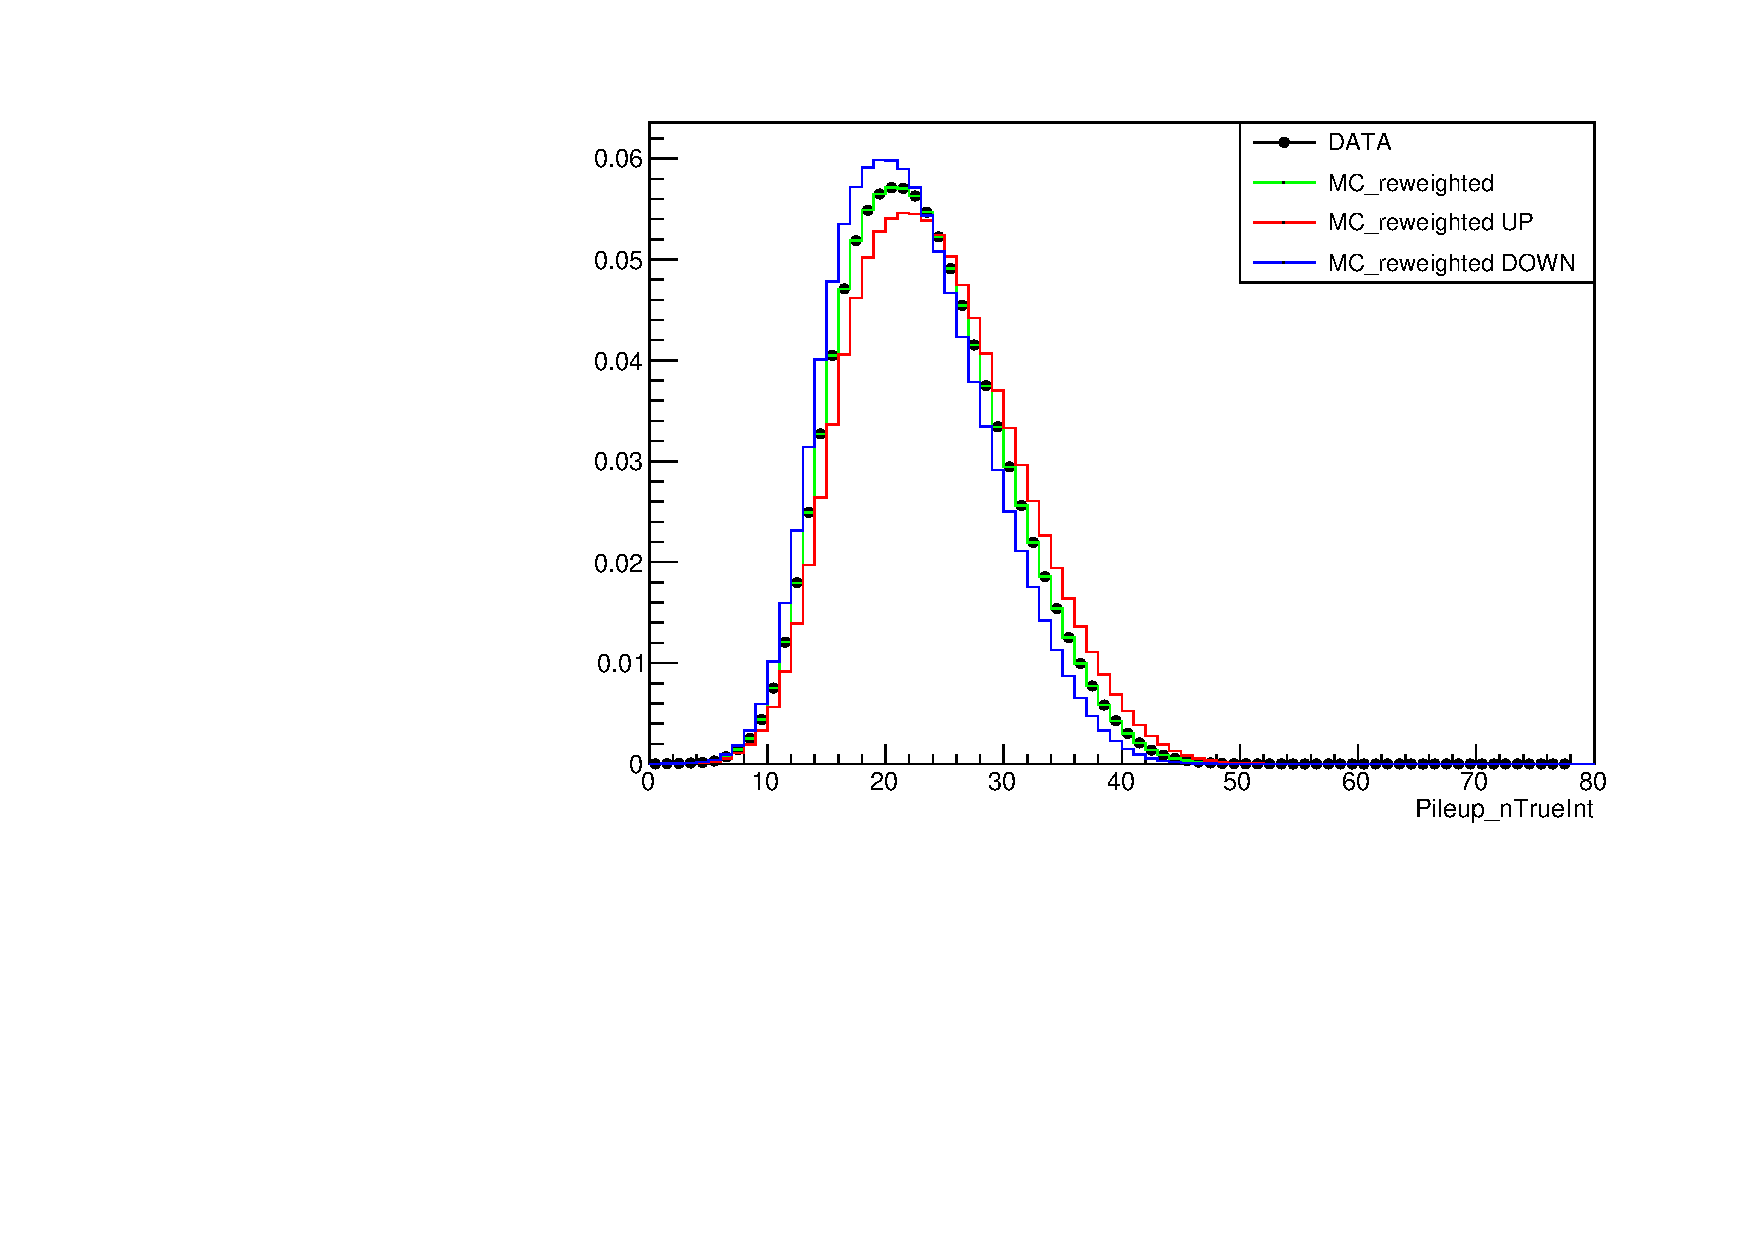
\includegraphics[width=0.55\textwidth]{figures/higgsmassmeas/Reweighted_2016.pdf}
    % 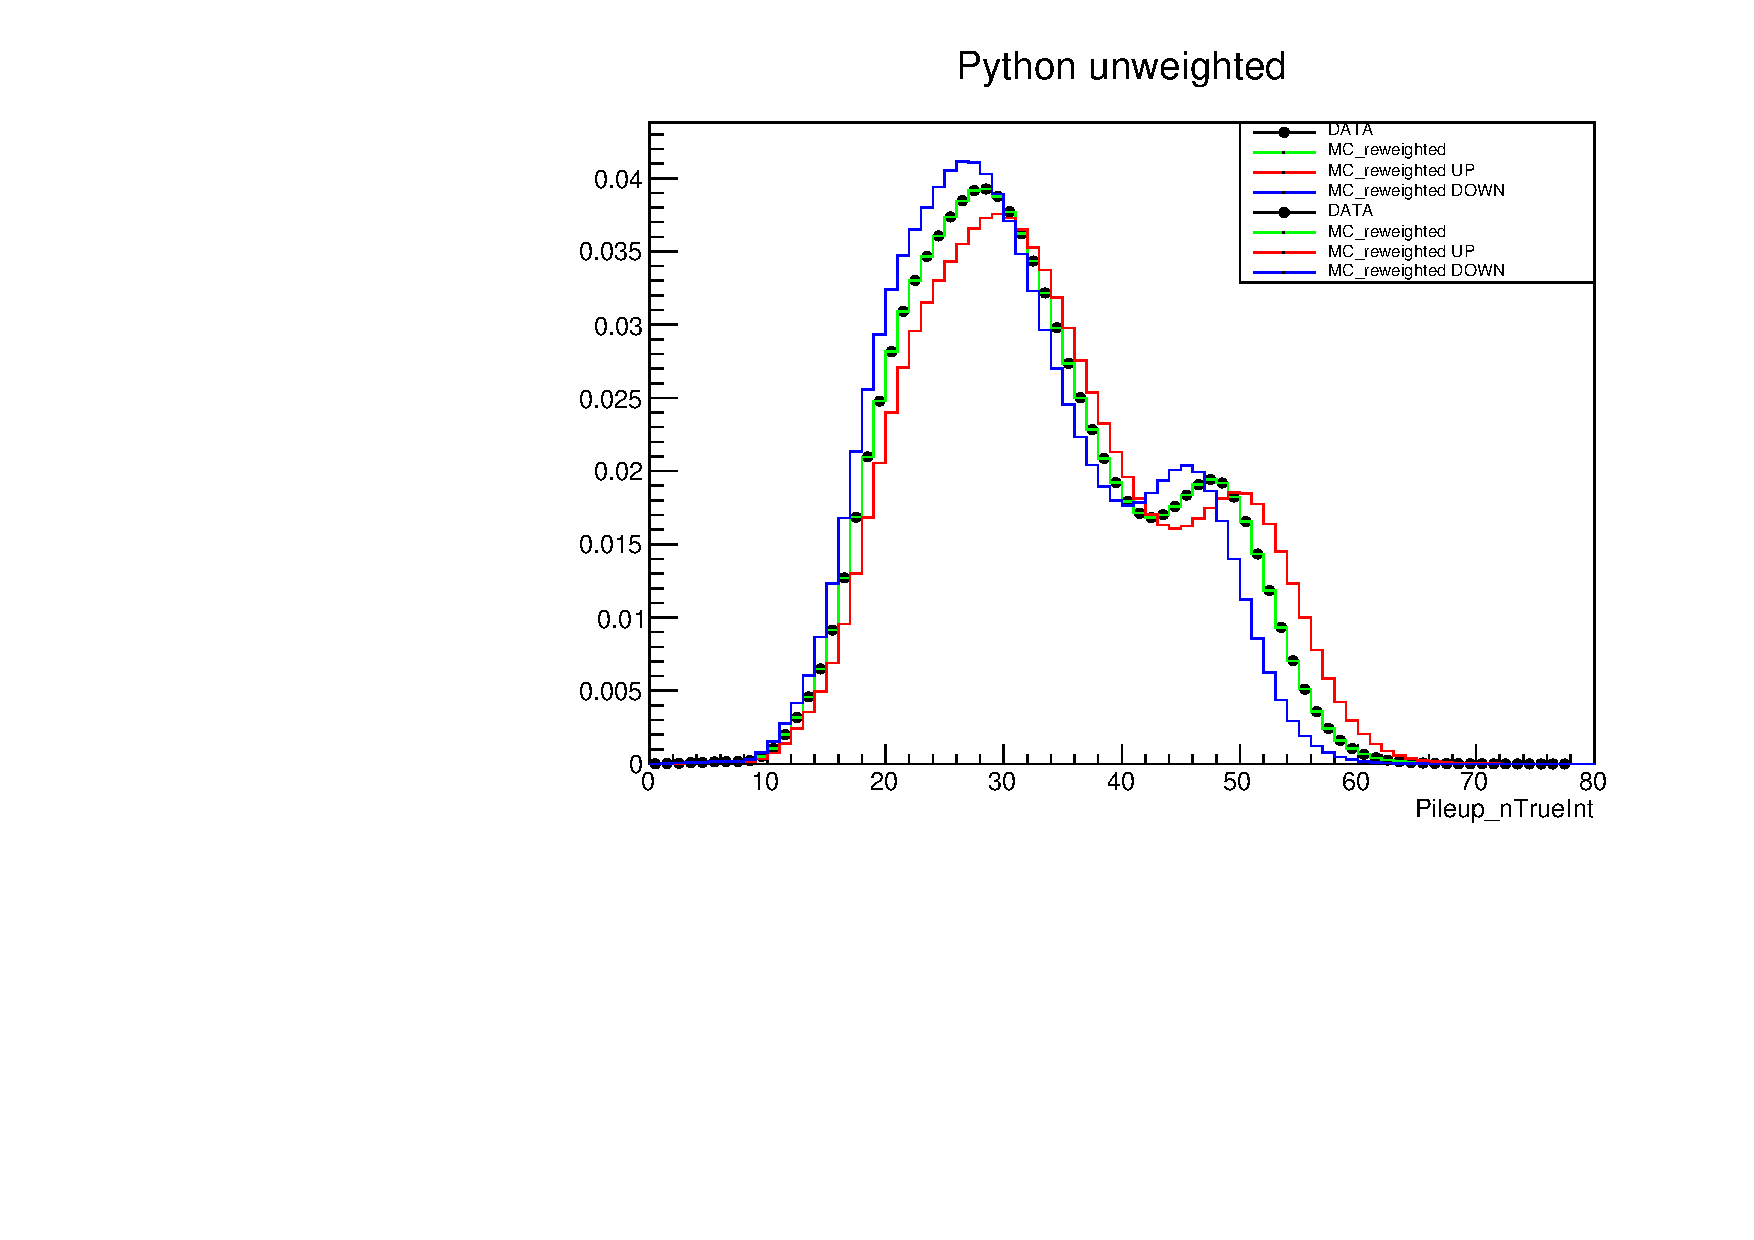
\includegraphics[width=0.55\textwidth]{figures/higgsmassmeas/Reweighted_2017.pdf}
    % 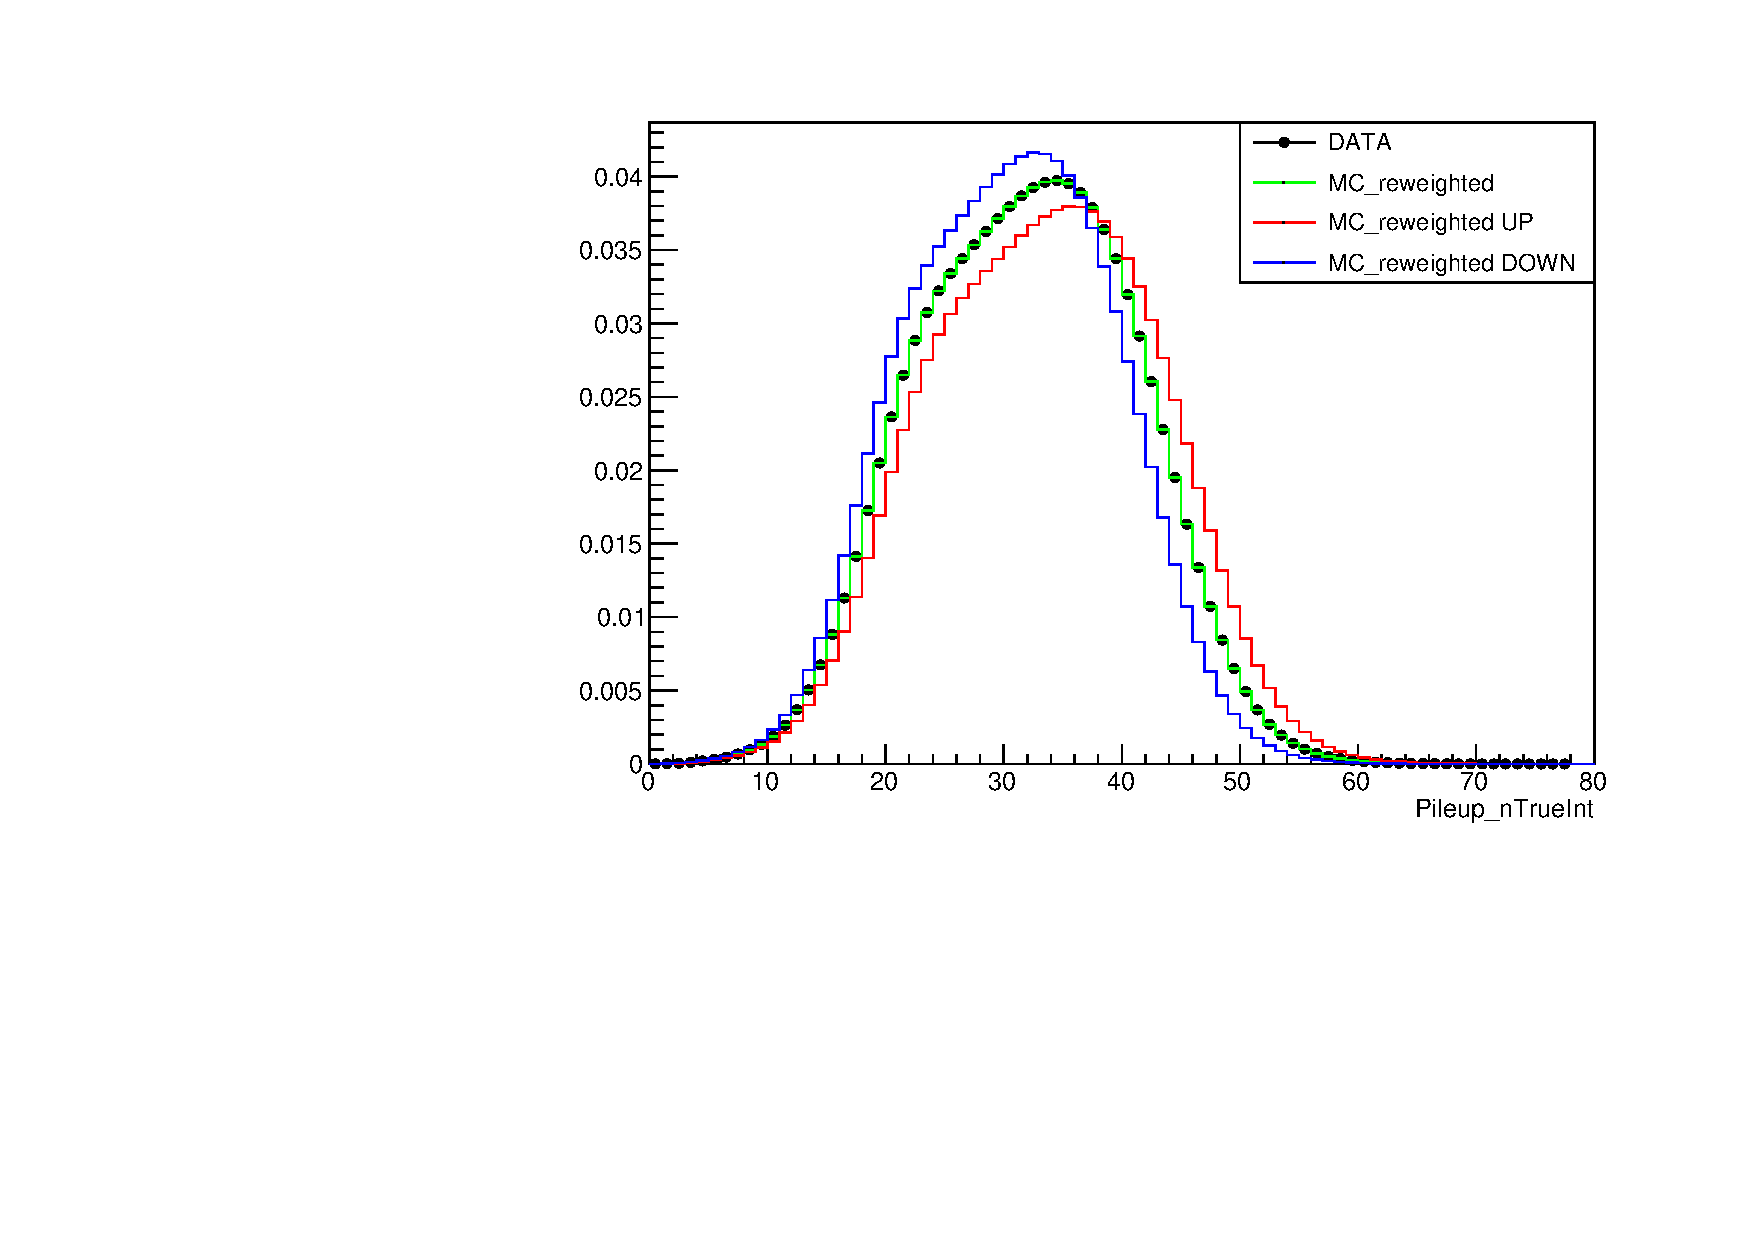
\includegraphics[width=0.55\textwidth]{figures/higgsmassmeas/Reweighted_2018.pdf}
    \addFigure{0.60}{figures/higgsmassmeas/Reweighted_2016.pdf}
    \addFigure{0.60}{figures/higgsmassmeas/Reweighted_2017.pdf}
    \addFigure{0.60}{figures/higgsmassmeas/Reweighted_2018.pdf}
    \captionof{figure}
        [words]
        {TODO:REWORD Data--simulation pileUp distributions: left 2016 (for pre and post-VFP), right 2017, bottom 2018. Up (down) scale has been obtained using 72.4 (66)\mb.}
    \label{fig:pileUpReweight}
\end{multiFigure}
